% Owner: B
We compare the country Louvain communities with UN regions in
Table~\ref{tab:regions}, the contingency table described in the analysis.
The majority share is the fraction of countries in a
community that belong to its most frequent region.

\begin{table}[h]
\centering
\small
\setlength{\tabcolsep}{4pt}
\begin{tabular}{@{}r r l c l@{}}
\toprule
Community & Size & Majority region & Share & Region counts \\
\midrule
0 & 49 & Europe & $31/49$ & Eu 31, Am 9, Af 4, As 3, Oc 2 \\
1 & 42 & Africa & $24/42$ & Af 24, Am 11, As 4, Eu 3 \\
2 & 32 & Asia & $21/32$ & As 21, Af 8, Eu 2, Am 1 \\
3 & 25 & Americas & $13/25$ & Am 13, Af 5, As 5, Oc 2 \\
4 & 9 & Asia & $9/9$ & As 9 \\
5 & 6 & Oceania & $5/6$ & Oc 5, Af 1 \\
6 & 3 & Oceania & $2/3$ & Oc 2, Af 1 \\
7 & 2 & Africa & $2/2$ & Af 2 \\
8 & 1 & Americas & $1/1$ & Am 1 \\
9 & 1 & Asia & $1/1$ & As 1 \\
10 & 1 & Oceania & $1/1$ & Oc 1 \\
\bottomrule
\end{tabular}
\caption{Country communities and UN regions. Shares are exact fractions.
Af = Africa, Am = Americas, As = Asia, Eu = Europe, Oc = Oceania;
omitted regions have no members. A majority region does not describe every
country in a mixed community.}
\label{tab:regions}
\end{table}

We find clear regional blocks: community $4$ contains $9$ Asian countries
out of $9$, and community $5$ contains $5$ countries in Oceania out of $6$.
The largest communities are mixed. Community $0$ contains $31$ European
countries and $9$ in the Americas, alongside other regions. Community $1$
contains $24$ African countries and $11$ in the Americas. We therefore do
not read the partition as a division into regions. Communities of sizes
$1$--$3$ partly reflect small dish profiles, which offer few ingredients
for comparing countries.

\paragraph{Shuffle test.}
Observed agreement is $0.643$, compared with a shuffled mean of $0.340$
and standard deviation $0.019$. The maximum over $1{,}000$ shuffles is
$0.404$, below the observed value (Figure~\ref{fig:shuffle}). No shuffle
reaches the observed agreement, giving $p=\frac{1}{1{,}001}\approx0.001$ with the
correction described in the analysis. Communities and UN regions are
therefore associated well beyond chance. This shows association, not cause,
and neighbouring countries are not independent.

\begin{figure}[h]
\centering
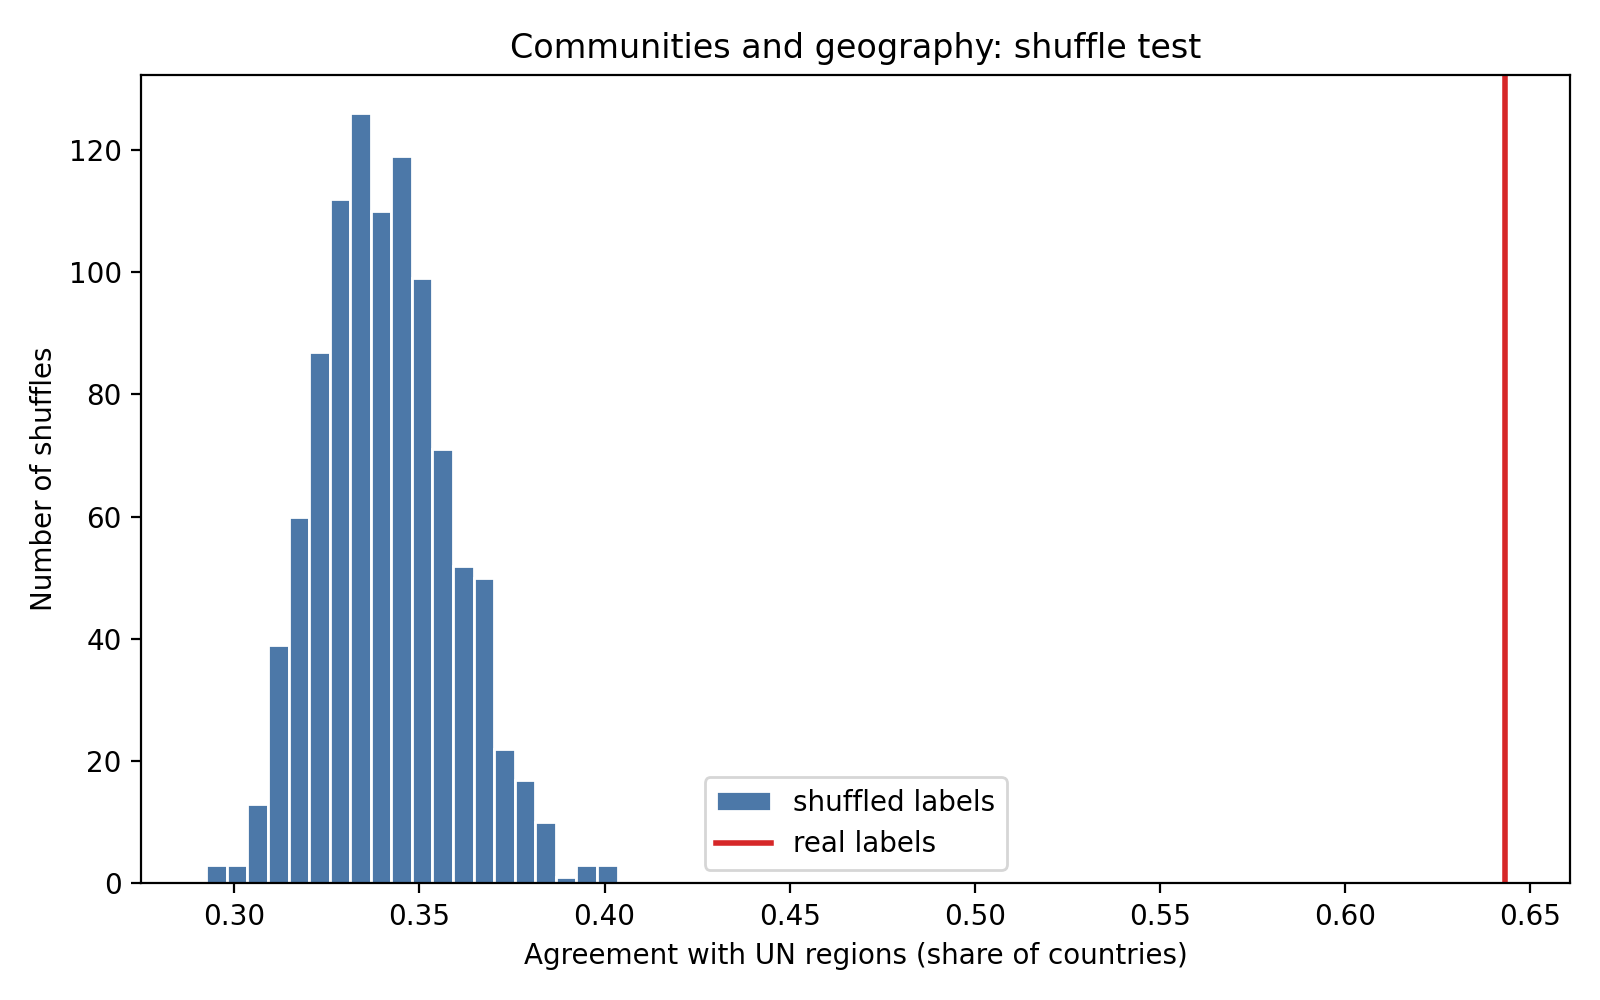
\includegraphics[width=0.75\linewidth]{shuffle_test.png}
\caption{Agreement with UN regions for the fixed Louvain communities:
1{,}000 shuffles of the region labels (bars) against the real labels (red line).}
\label{fig:shuffle}
\end{figure}

\paragraph{Connecting countries.}
Tonga, Fiji, Uganda, Mauritius and Tuvalu have the highest hop
betweenness. Betweenness follows degree less closely than for ingredients
($\rho=0.816$, against $0.973$), and the leaders are of two kinds. Fiji,
Uganda and Mauritius have many neighbours ($48$, $71$ and $66$), and most of
them lie in other communities ($62.5\%$, $76.1\%$ and $57.6\%$). These
outside neighbours span several regions: for Uganda, $26$ are in Africa,
$14$ in Asia, $8$ in the Americas and $6$ in Europe. These countries sit
between communities. Tonga and Tuvalu have only $9$ and $7$ neighbours.
Their betweenness comes from the bridges described below: every path from
Samoa passes through Tonga, and every path from Micronesia, Palau and
Seychelles passes through Tuvalu. Their rank therefore depends on small
profiles and on the threshold, like the cut points.

\paragraph{Cut points and small components.}
We find $5$ articulation points and $5$ bridges. Canada, Nicaragua and Samoa
each have a single neighbour (Belarus, Costa Rica and Tonga), so each hangs
on the rest of the graph by one bridge. Micronesia (Federated States of),
Palau and Seychelles form a small group attached only through the bridge
between Micronesia and Tuvalu. Outside the largest connected component,
Zambia and Zimbabwe form a component of two, and Grenada, Jordan and the
Marshall Islands are isolated. These countries have small dish profiles,
so a few ingredients decide whether they pass the Jaccard threshold of
$0.30$. We read these cut points as effects of the data and the threshold,
not as separations between cuisines.
